\section{SPC - Statistische Prozess- und Qualitätskontrolle}

\subsection{Einleitung}
\begin{itemize}
	\item Qualität = Gebrauchstauglichkeit
	\begin{itemize}
		\item Umgekehrt Proportional zur Variabilität
	\end{itemize}
	\item Wichtigste Tool: Die glorreichen Sieben
	\begin{itemize}
		\item[1.] Histogramm
		\item[2.] Check-Sheet (siehe Kapitel \ref{subsubsec:Kontrollblatt})
		\item[3.] Defect Concentration Diagramm (siehe Kapitel \ref{subsubsec:DefectConcentrationDiagramm})
		\item[4.] Pareto Chart (siehe Kapitel \ref{subsubsec:ParetoChart})
		\item[5.] Cause-and-Effect Diagramm (siehe Kapitel \ref{subsubsec:UrsacheWirkungsDiagramm})
		\item[6.] Kontrollkarte (siehe Kapitel \ref{subsec:Kontrollkarte})
		\item[7.] Streudiagramm
	\end{itemize}
\end{itemize}

\subsection{Basics}
\begin{itemize}
	\item Mittelwert mehrer Messwerte wird mit einem Querstrich bezeichnet, siehe z.B. Formel \ref{eq:Kontrollkarte1}.
	\item Ein geschätzer wert wird mit $\hat{ }$ bezeichnet (z.B. $\hat{\sigma}$
	\begin{itemize}
		\item Der exakte Wert ist nicht bekannt, wir schätzen mit werten aus der Vergangenheit
	\end{itemize}
	\item Nullhypothese $H_0$
	\begin{itemize}
		\item Annahme der 0-Hypothese: Prozess ist unter Kontrolle
		\item Ablehunung der 0-Hypothese: Prozess ist nicht unter Kontrolle
	\end{itemize}
\end{itemize}


\subsubsection{Kontrollblatt (Check-Sheet)}
\label{subsubsec:Kontrollblatt}
\begin{itemize}
	\item Formular zur Registrierung und Zählung möglicher Probleme
	\item Erfasst Ursachen und deren Auftreten für ein bestimmtes Ereignis (kann auch über verschiedene Zeitpunkte gemacht werden)
	\item Beispiel siehe Tabelle \ref{tab:CheckSheet}
\end{itemize}

\begin{table}[h!]
	\centering
	\begin{tabular}{l | c c c c | c}
		Ursachen					& \multicolumn{4}{c}{Unterbrechungen pro Quartal} 	&\\
									&1.		&2.		& 3.	&4.							&total\\\hline
		Telefon fallen lassen		&1		&0		&0		&2							&3\\
		Akku leer					&3		&3		&2		&4							&12\\
		Tunnelfahrt					&12		&10		&13		&9							&44\\
		Taste gedrückt				&1		&1		&0		&3							&5\\
		Unfall produziert			&1		&0		&0		&0							&1\\
		Telefon kaputt				&1		&0		&2		&1							&4\\
		kein offensichtlicher Grund	&3		&4		&3		&5							&15
	\end{tabular}
	\label{tab:CheckSheet}
	\caption{Beispiel eines Kontrollblattes \textit{Quelle:} \cite{C:CurtisSkriptCause}}
\end{table}


\subsubsection{Defect Concentration Diagramm}
\label{subsubsec:DefectConcentrationDiagramm}
\begin{itemize}
	\item Grafisches Pendant zum Kontrollblatt
	\item Auch Location Plot genannt
	\item Zeigt grafisch Orte des Auftretens verschiedener Fehler (Beispiel: Abbildung \ref{fig:DefectConcentration}
\end{itemize}
\begin{figure}[!h]
	\centering
	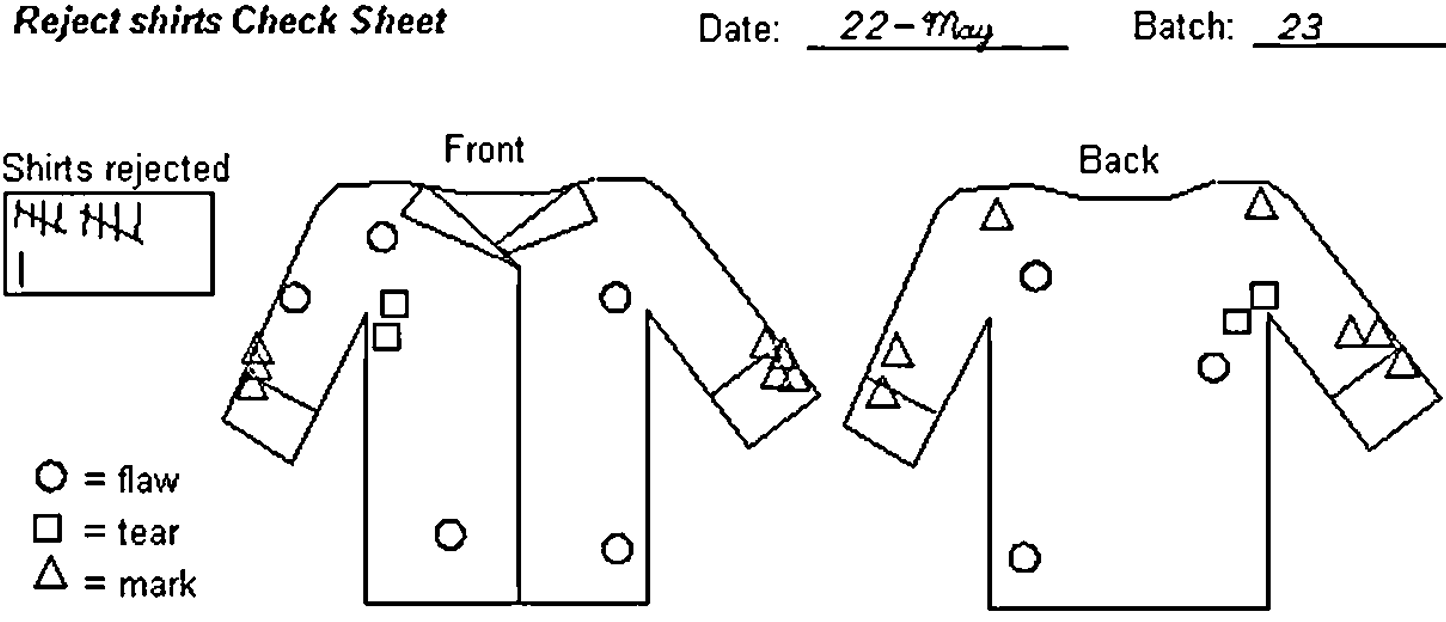
\includegraphics[width=0.5\linewidth]{figures/DefectConcentration}
	\caption{Ein Defect Concentration Diagramm \textit{Quelle:}\cite{C:DefectConcentration}}
	\label{fig:DefectConcentration}
\end{figure}

\subsubsection{Pareto-Chart}
\label{subsubsec:ParetoChart}
\begin{itemize}
	\item Bekannter unter dem Namen \glqq 80-20-Prinzip\grqq
	\begin{itemize}
		\item Wie viel Prozent des Resultats werden mit wie vielen Prozent des Einsatzes erreicht?
	\end{itemize}
	\item Mit einem kleinen Teil der eingesetzten Mittel bereits eine grosse Wirkung erzielen
	\item Pareto-Chart ist eine Spezielle Art des Histrogramms
	\begin{itemize}
		\item Histogramm und im gleichen Plott (auch auf gleicher Achsskalierung) die Summe aller bis zu diesem Punkt eingetragenen Histogramm-Werten
	\end{itemize}
\end{itemize}
\begin{figure}[!h]
	\centering
	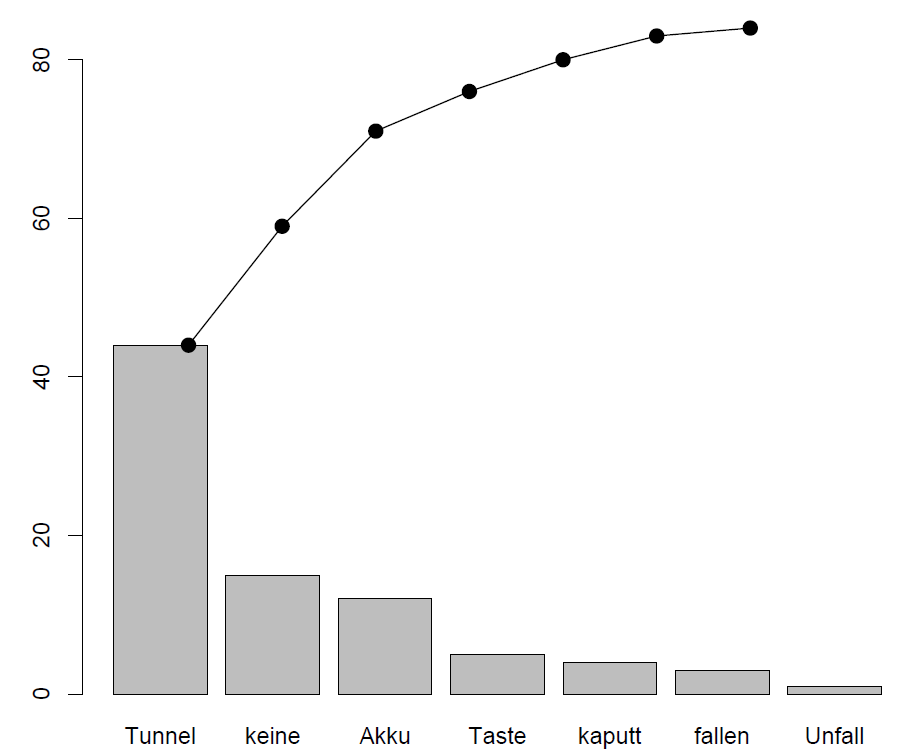
\includegraphics[width=0.3\linewidth]{figures/Pareto}
	\caption{Ein Pareto-Diagramm \textit{Quelle:}\cite{C:Pareto}}
	\label{fig:Pareto}
\end{figure}

\subsubsection{Ursache-Wirkungsdiagramm (Cause-and-Effect Diagramm)}
\label{subsubsec:UrsacheWirkungsDiagramm}
\begin{itemize}
	\item \glqq Fishbone-Diagramm\grqq 
	\item Grafische Strukturierung des Problems für übersichtliche Gesamtbetrachtung
	\item Der Kopf des Fisches stellt das Ziel dar
	\item Folgende Bereiche können gut als \glqq Top-Level-Fischgräte\grqq verwendet werden (jeweils inkl. Beispielen)
	\begin{itemize}
		\item Ausrüstung \textit{Software, Büroplatz, etc.}
		\item Umwelt \textit{Lärm, Hitze, etc.}
		\item Menschen \textit{Ausbildung, Motivation, etc.}
		\item Maschinen \textit{Bedienung, Alter, etc}
		\item Materialien \textit{Qualität, Beschaffung, etc.}
		\item Methoden \textit{Bestellung, Standartisierung, etc.}
	\end{itemize}
\end{itemize}

\subsection{Kontrollkarte}
\label{subsec:Kontrollkarte}
Die Grundlage einer Kontrollkarte bildet der statistische Test zur Prüfung einer statistischen Hypothese
\subsubsection{Basics}
\begin{itemize}
	\item $X$: Ein Zufallsvariabel
	\item $\mu_0$: Zielwert (gemäss Vorgabe, z.B. Fertigungszeichnung)
	\item $\mu_1$: Effektiver Mittelwert des gemessenen Parameters
	\item $\mu$: Wert des gemessenen Parameters
	\item $\delta_{1,2}$: Untere, resp. Obere Toleranzgrenze
	\item $\sigma^2$: Varianz
	\item $\sigma$: Standardabweichung
	\item $\bar{x}$: Aus Stichproben errechneter Mittelwert
	\item Standardfehler $=\frac{\sigma}{\sqrt{n}} = \sigma(\bar{X})$
	\item USL = Upper Specification Limit $\Rightarrow \mu_0+\delta_2$
	\item LSL = Lower Specification Limit $\Rightarrow \mu_0+\delta_1$
	\begin{itemize}
		\item Der durch UCL und LCL begrenzte Bereich heisst Kontrollbereich
	\end{itemize}
	\item $H_0$ Nullhypothese
	\begin{itemize}
		\item Annahme von $H_0$ Prozess ist unter Kontrolle (LCL $\leq \bar{x} \leq$ UCL)
	\end{itemize}
	\item Einem Test zu $n$ Zeitpunkten eine Serie von $m$ Proben entnehmen um die Zufallsvariabel $X$ zu bestimmen
	\begin{itemize}
		\item [$\rightarrow$] $n$ mal einen Versuch mit jeweils $m$ Proben (auf die gleiche Eigenschaft) geben $n$ Realisierungen der Variabel $X$
	\end{itemize}
	\item $z_q$: Quantil der Normalverteilung (siehe Tafel \ref{Anh:TafelqQuantileStandardisierteNormalverteilung}
	\begin{itemize}
		\item $\alpha$ Vorgegeben Irtumswahrscheinlichkeit $\in \left[0,0.5\right]$
		\item $z_q$ ist die Abweichung in $\sigma$ von $\mu_0$ 
		\item $P(Z\leq z_q =1-\frac{\alpha}{2}$ anhand von $\alpha$ das Zugehörige $q$ in Tabelle \ref{Anh:TafelqQuantileStandardisierteNormalverteilung} suchen
	\end{itemize}
	\item UCL und LCL entsprechend der Formel \ref{eq:UCLLCL1}  berechnen
	\begin{itemize}
		\item Mit dieser Formel berechnet sich aus der Streuung die zulässigen Toleranzbänder, damit ein gewisser Prozentsatz der Teile innerhalb dieses Bandes ist. 
	\end{itemize}
\end{itemize}
\begin{equation}
	\label{eq:UCLLCL1}
	\text{UCL} = \mu_0 + z_q\frac{\sigma}{\sqrt{n}} \qquad \text{und} \qquad
	\text{LCL} = \mu_0 - z_q\frac{\sigma}{\sqrt{n}}
\end{equation}

\subsubsection{Shewhart Kontrollkarte}
\begin{itemize}
	\item Da die Prozessstreuung meist unbekannt ist, muss diese aus einem Vorlauf geschätzt werden. 
	\item Die Karten werden in Paaren gebraucht (z.B. eine für Mittelwert, eine für Streuung)
	\item Ein Beispiel für die Datenaufnahem ist in Tabelle \ref{tab:RSKarte} gezeigt
	\begin{itemize}
		\item Es werden $k$ Stichproben gemacht (sog. Gruppen) mit jeweils $n$ Werten
	\end{itemize}
	\item Die Spannweite ist die Differenz zwischen minimalem und maximalen Wert einer Gruppe
	\item Die elementaren Formeln sind \ref{eq:Kontrollkarte1} und \ref{eq:Kontrollkarte2} gezeigt
\end{itemize}
\begin{table}[!h]
	\centering
	\begin{tabular}{c |c c c c cc|c|c|c}
		Stichprobe	& \multicolumn{6}{c|}{Stichprobenwert} & Mittelwert 	& Standardabweichung &Spannweite\\\hline
		1			&$x_{11}$&$x_{12}$&$\ldots$&$x_{1j}$&$\ldots$&$x_{1n}$&$\bar{x}_1$	&$s_1$	&$R_1$\\
		2			&$x_{21}$&$x_{22}$&$\ldots$&$x_{2j}$&$\ldots$&$x_{2n}$&$\bar{x}_2$	&$s_2$	&$R_2$\\
		$\vdots$	&$\vdots$&$\vdots$& 	   &$\vdots$&		 &$\vdots$&$\vdots$		&$\vdots$&$\vdots$\\
		i			&$x_{i1}$&$x_{i2}$&$\ldots$&$x_{ij}$&$\ldots$&$x_{in}$&$\bar{x}_i$	&$s_i$	&$R_i$\\
		$\vdots$	&$\vdots$&$\vdots$& 	   &$\vdots$&		 &$\vdots$&$\vdots$		&$\vdots$&$\vdots$\\
		k			&$x_{k1}$&$x_{k2}$&$\ldots$&$x_{kj}$&$\ldots$&$x_{kn}$&$\bar{x}_k$	&$s_k$	&$R_k$\\
	\end{tabular}
	\caption{Beispiel für $k$ Stichproben (Gruppen) mit jeweils $n$ Werten \textit{Quelle:}\cite{C:RSKarte}}
	\label{tab:RSKarte}
\end{table}
\begin{align}
	\label{eq:Kontrollkarte1}
	\bar{x}_i = \frac{1}{n}\sum_{j=1}^{n}x_{ij} \qquad \text{und} \qquad s_i=\sqrt{\frac{1}{n-1}\sum_{j=1}^{n}\left(x_{ij}-\bar{x}_i\right)^2}\\
	\label{eq:Kontrollkarte2}
	R_i = \max\left\lbrace x_{ij}\vert j\in \left\lbrace 1,\ldots,n\right\rbrace\right\rbrace - \min\left\lbrace x_{ij}\vert j\in \left\lbrace 1,\ldots,n\right\rbrace\right\rbrace
\end{align}

\subsubsection{$\bar{x}$ und $R$-Karte}
\begin{itemize}
	\item Für die Konstruktion der Karte werden $k$ Daten aus dem Vorlauf benutzt
	\item Die horizontale Achse der Karten ist jeweils der Index $i$, die vertikale Achse ist: 
	\begin{itemize}
		\item Spannweite bei der $R$-Karte
		\item Mittelwert bei der $\bar{x}$-Karte
	\end{itemize}
	\item Prozessstreuung zuerst unter Kontrolle bringen, danach die $\bar{x}$-Karte konstruieren
	\item Die Mittellinie (CL) der $R$-Karte wird mit $\bar{R}$ bezeichnet und berechnet sich gemäss Formel \ref{eq:xRKarte}
	\item Die Standardabweichung von $\bar{R}$ ist $\sigma_R$
	\item Wenn $\sigma_R$ normalverteilt ist, kann:
	\begin{itemize}
		\item für $\text{UCL}_R = D_4\bar{R}$ genommen werden
		\item für $\text{LCL}_R = D_3\bar{R}$ genommen werden
		\item $D_3$ und $D_4$ stammen von Anhang \ref{Anh:TafelFaktorenKontrollkarten} und hängen vom Stichprobenumfang $n$ ab
	\end{itemize}
	\item Vorgehen:
	\begin{itemize}
		\item [1.] Mittellinie, LCL und UCL in Karte eintragen
		\item [2.] Spannweiten $R_i$ eintragen im Streudiagramm eintragen
		\item Wenn Stichproben ausserhalb der Grenzen liegen, diese Messungen weglassen und Grenzen neu berechnen
	\end{itemize}
	\item Wenn $R$-Karte unter statistische Kontrolle ist, können für die Berechnung des UCL und des LCL auch die Formeln \ref{eq:xRKarte2} bis \ref{eq:xRKarte3} gebraucht werden
	\begin{itemize}
		\item Die Parameter $d_2$ und $A_2$ stammen aus Anhang \ref{Anh:TafelFaktorenKontrollkarten} und ist in Abhängigkeit der Anzahl Stichproben
		\item $\hat{\sigma}$ ist eine Schätzung für $\sigma$, siehe Formel \ref{eq:xRKarte4}
		\item $k^\ast$ bezeichnet Summe über alle gültigen Stichproben
	\end{itemize}
	\item Vorteil: Einfacher zu berechnen als $\bar{x}$-s-Karte
	\item \textbf{Formeln für die Berechnung von $\bar{x}$ und $R$-Karten}
\end{itemize}
\begin{align}
	\label{eq:xRKarte}
	\bar{R} &= \frac{1}{k}\sum_{i=1}^{k}R_i\\
	\label{eq:xRKarte4}
	\hat{\sigma} &= \frac{\bar{R}}{d_2}\\
	\label{eq:xRKarte2}
	\bar{\bar{x}} &= \frac{1}{k^\ast}\sum_{i=1}^{k^\ast}\bar{x}_i\\
	\label{eq:xRKarte3}
	\text{UCL}_{\bar{x}}  &= \bar{\bar{x}} + 3\frac{\bar{R}}{d_2\sqrt{n}} \approx \bar{\bar{x}}+A_2\bar{R} \qquad \text{und} \qquad \text{LCL}_{\bar{x}} = \bar{\bar{x}} - 3\frac{\bar{R}}{d_2\sqrt{n}} \approx \bar{\bar{x}}-A_2\bar{R}
\end{align}

\subsubsection{$\bar{x}$ und s-Karte}
\begin{itemize}
	\item Wie bei $\bar{x}$ und $R$-Karten zuerst die Streuung unter Kontrolle bringen
	\item Die horizontale Achse der Karten ist jeweils der Index $i$, die vertikale Achse ist: 
	\begin{itemize}
		\item Standardabweichung bei der $s$-Karte
		\item Mittelwert bei der $\bar{x}$-Karte
	\end{itemize}
	\item Parameter werden ebenfalls mit $k$ Stichproben aus einem Vorlauf berechnet
	\item Die Mittellinie ($\bar{s}$ ist das arithmetische Mittel aller Standardabweichungen des Vorlaufes
	\item UCL und LCL lassen sich mit $B_3$ und $B_4$ (aus Anhang \ref{Anh:TafelFaktorenKontrollkarten} berechnen
	\begin{itemize}
		\item $\text{UCL}_s = B_4\bar{s}$ und $\text{LCL}_s = B_3\bar{s}$
	\end{itemize}
	\item Vorteil der $\bar{x}$ und s-Karte: Nutzt vorhandene Informationen besser als $R$-$\bar{x}$-Karte
	\item \textbf{Formeln \ref{eq:xSKarte} bis \ref{eq:xSKarte3} für die Berechnung von $\bar{x}$ und $s$-Karten}
\end{itemize}
\begin{align}
	\label{eq:xSKarte}
	\bar{s} &= \frac{1}{k}\sum_{i=1}^{k}s_i\\
	\label{eq:xSKarte4}
	\hat{\sigma} &= \frac{\bar{s}}{c_4}\\
	\label{eq:xSKarte2}
	\bar{\bar{x}} &= \frac{1}{k^\ast}\sum_{i=1}^{k^\ast}\bar{x}_i\\
	\label{eq:xSKarte3}
	\text{UCL}_{\bar{x}} &= \bar{\bar{x}} + 3\frac{\bar{s}}{c_4\sqrt{n}} \approx \bar{\bar{x}}+A_3\bar{R} \qquad \text{und} \qquad \text{LCL}_{\bar{x}} = \bar{\bar{x}} - 3\frac{\bar{s}}{c_4\sqrt{n}} \approx \bar{\bar{x}}-A_4\bar{R}	
\end{align}

\subsubsection{Kontrollkarte für einzelne Messwerte}
\begin{itemize}
	\item Die horizontale Achse der Karten ist jeweils der Index $i$, die vertikale Achse ist: 
	\item Die vertikale Achse ist in der Einheit der gemessenen Grösse (z.b. \si{\milli\meter} und es werden gleich die gemessenen Grössen eingetragen
	\item Es gilt: Stichprobenumfang $n=1$
	\begin{itemize}
		\item Stichprobe besteht aus einer einzelnen Beobachtung
	\end{itemize} 
	\item Dies kann zur Anwendung kommen, wenn:
	\begin{itemize}
		\item Jedes produzierte Teil gemessen werden soll
		\item Die Produktion sehr viel Zeit in Anspruch nimmt
		\item Unterschied einer wiederholten Messung nicht auf die Prozessstreuung zurück zu führen ist. 
	\end{itemize}
	\item Die Kontrollkarte für einzelne Messwerte nutzt die gleitende Spannweite $\text{M}R_i$ zur Schätzung der Prozessstreuung 
	\item \textbf{Formeln \ref{eq:GleitendeSpannweite} bis \ref{eq:UCLLCLeinzelneMesswerte} für die Berechnung von Kontrollkarten für einzelne Messwerte}
\end{itemize}
\begin{align}
	\label{eq:GleitendeSpannweite}
	\text{M}R_i &=\left\lvert x_{i+1}-x_i \right\rvert\\
	\label{eq:MittelwertGleitendeSpannweite}
	\overline{\text{M}R} &= \frac{1}{n-1}\sum_{i=1}^{n-1}\text{M}R_i\\
	\label{eq:SchaetzungStreuung}
	\hat{\sigma} &= \frac{\overline{\text{M}R}}{d_2} = \frac{\overline{\text{M}R}}{1.128}\\
	\label{eq:UCLLCLeinzelneMesswerte}
	\text{UCL} &= \bar{x} + 3\frac{\overline{\text{M}R}}{1.128} \qquad \text{und} \qquad \text{LCL} = \bar{x} - 3\frac{\overline{\text{M}R}}{1.128}
\end{align}

\subsubsection{Die $P$-Kontrollkarte für relative Häufigkeiten}
\begin{itemize}
	\item Entgegen der anderen Kontrollkarten, wird für diese nur geprüft und nicht gemessen (entweder ist Anforderung erfüllt oder nicht)
	\item Somit braucht es Kontrollkarten für relative Häufigkeit 
	\item Benötigt grossen Stichprobenumfang
	\item $n$ der Stichprobenumfang in welchem wir $D$ defekte Teile finden
	\begin{itemize}
		\item $D$ ist binominalverteilt in $n$
		\item Verteilung hat unbekannte Erfolgswahrscheinlichkeit $p$
	\end{itemize}
	\item Relative Häufigkeit der Defekten Teile: Formel \ref{eq:RelHaeufigkeit}
	\item Varianz dieser Erfolgswahrscheinlichkeit Formel \ref{eq:VarianzRelHaeufigkeit}
	\item Die Erfolgswahrscheinlichkeit der $k$ einzelnen Stichproben als Formel \ref{eq:RelHaeufigkeitMultiple}
	\item Wenn alle $k^\ast$ gültigen Strichproben den gleichen Umfang haben:
	\begin{itemize}
		\item Formel \ref{eq:RelhaeufigkeitCL} für Mittellinie (Mittelwert der Wahrscheinlichkeiten)
		\item Formel \ref{eq:RelHaeufigUCLLCL} für die Kontrollgrenzen
	\end{itemize} 
	\item Wenn nicht alle $k^\ast$ Strichproben den gleichen Umfang haben:
	\begin{itemize}
		\item Formel \ref{eq:RelhaeufigkeitCL2} für Mittellinie (Mittelwert der Wahrscheinlichkeiten)
		\item Formel \ref{eq:RelHaeufigUCLLCL2} für die Kontrollgrenzen
		\item \textbf{Achtung:} Jetzt ist UCL und LCL von der Anzahl Proben abhängig und das Toleranzband muss nicht mehr unbedingt eine gerade Linie darstellen.
	\end{itemize} 
	\item Bei kleinen Stichprobenumfängen kann es sein, dass LCL negativ wird, in diesem Fall LCL=0 nehmen
	\item Vorteil: Günstig und einfach, Nachteil: Grosser Stichprobenumfang nötig
	\item \textbf{Formeln \ref{eq:RelHaeufigkeit} bis \ref{eq:RelHaeufigUCLLCL2} für die Berechnung von Kontrollkarten mit relativer Häufigkeit}
	\item $\hat{\sigma}$ kann geschätzt werden mit $\hat{\sigma}=\frac{\bar{s}}{c_4}$
	\begin{itemize}
		\item $c_4$ aus Anhang \ref{Anh:TafelFaktorenKontrollkarten}
	\end{itemize}
\end{itemize}
\begin{align}
	\label{eq:RelHaeufigkeit}
	\hat{p} &= \frac{D}{n}\\
	\label{eq:VarianzRelHaeufigkeit}
	\text{Var}\left(\hat{p}\right) &= \frac{p(1-p}{n}\\
	\label{eq:RelHaeufigkeitMultiple}
	p_1 &= \frac{d_1}{n_1},\ldots,p_k = \frac{d_k}{n_k}\\
	\label{eq:RelhaeufigkeitCL}
	\bar{p}&=\frac{1}{k^\ast}\sum_{i=1}^{k^\ast}p_i\\
	\label{eq:RelHaeufigUCLLCL}
	\text{UCL} &= \bar{p}+3\sqrt{\frac{\bar{p}(1-\bar{p}}{n}}		\qquad \text{und}\qquad
	\text{LCL} = \bar{p}-3\sqrt{\frac{\bar{p}(1-\bar{p}}{n}}\\
	\label{eq:RelhaeufigkeitCL2}	
	\bar{p}&= \frac{d_1+\cdots +d_{k^\ast}}{n_1+\cdots +n_{k^\ast}}\\
	\label{eq:RelHaeufigUCLLCL2}
	\text{UCL}_i &= \bar{p}+3\sqrt{\frac{\bar{p}(1-\bar{p}}{n_i}}		\qquad \text{und}\qquad
	\text{LCL}_i = \bar{p}-3\sqrt{\frac{\bar{p}(1-\bar{p}}{n_i}}\\
\end{align}
\clearpage